\chapter{Instant Insanity Puzzle}

Rishnak was examining the headstones of some of the graves and came across a headstone with the name Schossow\footnote{Frederick Schossow received a patent in 1900 for proposing this puzzle in 1899, as described here: \url{https://patents.google.com/patent/US646463A/en}.} on a grave. Memories of this puzzle flooded Rishnak's senses. Schossow's puzzle had card suits (i.e.,~hearts, diamonds, clubs, and spades) marked on each face. In 1967, Frank Armbruster created a variation of this puzzle with colors instead of suits, which was published by Parker Brothers---that puzzle was called the ``instant insanity'' puzzle.

Rishnak thought this puzzle, with its graph-theoretic solution, would certainly appeal to Ajur. It did not take long for Rishnak to find Ajur and Jura.

Excitedly, Rishnak said, ``For our last day, we are going to talk about one of my favorite puzzles. This puzzle has a long solution that uses search techniques and a short solution that we can explore using some clever graph theory techniques.''

Ajur, seeing Rishnak's enthusiasm, said, ``Sure, what's the puzzle?''

Rishnak continued, ``The puzzle itself consists of four cubes numbered~$1,2,3,4$, with each face colored as shown in front of you.'' Rishnak waved his hands and a colorful display of cubes floated in front of Ajur [Figure~\ref{22p1}]. \index{instant insanity puzzle}

\begin{newpage}
\end{newpage}
\begin{figure}
\begin{center}
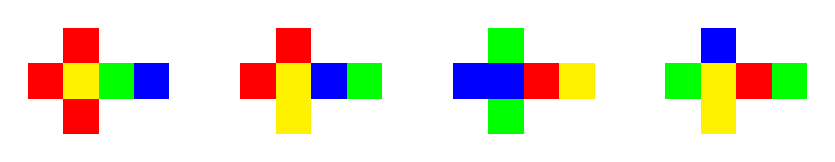
\begin{tikzpicture}
[scale=.9]
%First Cube
\fill [red] (0.0,0.0) rectangle (0.5,0.5);
\fill [yellow] (0.5,0.0) rectangle (1.0,0.5);
\fill [green] (1.0,0.0) rectangle (1.5,0.5);
\fill [blue] (1.5,0.0) rectangle (2.0,0.5);
\fill [red] (0.5,-0.5) rectangle (1.0,0.0);
\fill [red] (0.5,0.5) rectangle (1.0,1.0);
%Second Cube
\fill [red] (3.0,0.0) rectangle (3.5,0.5);
\fill [yellow] (3.5,0.0) rectangle (4.0,0.5);
\fill [blue] (4.0,0.0) rectangle (4.5,0.5);
\fill [green] (4.5,0.0) rectangle (5.0,0.5);
\fill [yellow] (3.5,-0.5) rectangle (4.0,0.0);
\fill [red] (3.5,0.5) rectangle (4.0,1.0);
%Third  Cube
\fill [blue] (6.0,0.0) rectangle (6.5,0.5);
\fill [blue] (6.5,0.0) rectangle (7.0,0.5);
\fill [red] (7.0,0.0) rectangle (7.5,0.5);
\fill [yellow] (7.5,0.0) rectangle (8.0,0.5);
\fill [green] (6.5,-0.5) rectangle (7.0,0.0);
\fill [green] (6.5,0.5) rectangle (7.0,1.0);
%Fourth Cube
\fill [green] (9.0,0.0) rectangle (9.5,0.5);
\fill [yellow] (9.5,0.0) rectangle (10.0,0.5);
\fill [red] (10.0,0.0) rectangle (10.5,0.5);
\fill [green] (10.5,0.0) rectangle (11.0,0.5);
\fill [yellow] (9.5,-0.5) rectangle (10.0,0.0);
\fill [blue] (9.5,0.5) rectangle (10.0,1.0);
\end{tikzpicture}
\caption{The four cubes that make up the instant insanity puzzle}\label{22p1}
\end{center}
\end{figure}

Rishnak said, ``The problem is to stack these four cubes vertically in a column such that all of the cubes on each side of the column (left, right, front, and back) have distinct colors. Here''---he flashed his hands and two cubes came together [Figure~\ref{22p2}]---``we have cube~4 sitting on top of cube~1. See that all faces have distinct colors?''

Ajur nodded. He asked, ``We need to do that with all four cubes?''

\begin{figure}
\begin{center}
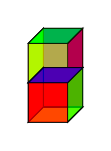
\begin{tikzpicture}
\coordinate (O) at (0,0,0);
\coordinate (A) at (0,0.5,0);
\coordinate (B) at (0,0.5,0.5);
\coordinate (C) at (0,0,0.5);
\coordinate (D) at (0.5,0,0);
\coordinate (E) at (0.5,0.5,0);
\coordinate (F) at (0.5,0.5,0.5);
\coordinate (G) at (0.5,0,0.5);

\draw[black,fill=yellow] (O) -- (C) -- (G) -- (D) -- cycle;% Bottom Face
\draw[black,fill=blue] (O) -- (A) -- (E) -- (D) -- cycle;% Back Face
\draw[black,fill=green] (O) -- (A) -- (B) -- (C) -- cycle;% Left Face
\draw[black,fill=red,opacity=0.7] (D) -- (E) -- (F) -- (G) --cycle;% Right Face
\draw[black,fill=yellow,opacity=0.7] (C) -- (B) -- (F) -- (G) --cycle;% Front Face
\draw[black,fill=green,opacity=0.7] (A) -- (B) -- (F) -- (E) -- cycle;% Top Face
\coordinate (OO) at (0,-0.5,0);
\coordinate (AA) at (0,0,0);
\coordinate (BB) at (0,0,0.5);
\coordinate (CC) at (0,-0.5,0.5);
\coordinate (DD) at (0.5,-0.5,0);
\coordinate (EE) at (0.5,0,0);
\coordinate (FF) at (0.5,0,0.5);
\coordinate (GG) at (0.5,-0.5,0.5);

\draw[black,fill=yellow] (OO) -- (CC) -- (GG) -- (DD) -- cycle;% Bottom Face
\draw[black,fill=red] (OO) -- (AA) -- (EE) -- (DD) -- cycle;% Back Face
\draw[black,fill=red] (OO) -- (AA) -- (BB) -- (CC) -- cycle;% Left Face
\draw[black,fill=green,opacity=0.7] (DD) -- (EE) -- (FF) -- (GG) --cycle;% Right Face
\draw[black,fill=red,opacity=0.7] (CC) -- (BB) -- (FF) -- (GG) --cycle;% Front Face
\draw[black,fill=blue,opacity=0.7] (AA) -- (BB) -- (FF) -- (EE) -- cycle;% Top Face
%% Following is for debugging purposes so you can see where the points are
%% These are last so that they show up on top
%\foreach \xy in {O, A, B, C, D, E, F, G}{
%    \node at (\xy) {\xy};
%}
\end{tikzpicture}
\caption{Cube~4 placed on top of cube~1 such that all faces have distinct colors}\label{22p2}
\end{center}
\end{figure}

Rishnak nodded, unable to stop himself from smiling. He said, ``If we start with a brute force solution, also known as an exhaustive search technique, then for each cube, we have to choose which face should be at the bottom of the cube. There are six possibilities to choose from. And once we have decided on the color of the bottom face, there are four rotations for the sides of the cube. Therefore, we have~24 possibilities for each cube.''

Ajur caught on quickly. He said, ``And with four cubes to be stacked, that means we have~$24\times 24\times 24\times 24$ possibilities.''

Rishnak said, ``Correct, or~$24^4$, which equals~$331,776$ possibilities. By searching each of these~$331,776$ possibilities, we will find a solution and---''

Ajur said, ``Wait, for the bottom cube, we don't need to consider the four rotations. Instead, we can fix that cube in place.''

Rishnak smiled, impressed with Ajur's quickness. Rishnak continued, ``And if we find one solution, then we can also permute the cube positions without altering the constraints to find other solutions. We could consider three opposite faces of each cube. There are four colors---red, yellow, green, and blue---so these form the vertices. Two vertices (or colors) are adjacent if they form the opposite sides of the same cube.''

Ajur was puzzled, so Rishnak waved his hands and showed an example graph [Figure~\ref{22g1}]. Rishnak said, ``This graph represents the first cube.'' He waved his hands again and again, forming three other graphs [Figure~\ref{22g2}] [Figure~\ref{22g3}] [Figure~\ref{22g4}], then said, ``Similarly, we can draw graphs for each of the other cubes.''

\begin{figure}[h]
\begin{center}
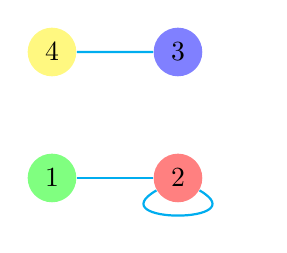
\begin{tikzpicture}
  [scale=.4,auto=left,every node/.style={circle}]
\node (n1)[fill=blue!50] at (4,4) {3};
  \node (n2)[fill=green!50] at (0,0)  {1};
  \node (n3)[fill=red!50] at (4,0)  {2};
  \node (n4)[fill=yellow!50] at (0,4)  {4};;
 \foreach \from/\to in {n3/n2,n1/n4}
    \draw[cyan,thick] (\from) -- (\to);
  \draw[cyan,thick]
  (n3) to[out=210,in=330,looseness=4] (n3);
\end{tikzpicture}
\caption{The graph representing cube~1}\label{22g1}
\end{center}
\end{figure}

\begin{figure}[h]
\begin{center}
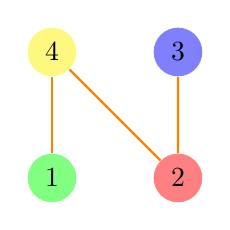
\begin{tikzpicture}
  [scale=.4,auto=left,every node/.style={circle}]
 \node (n1)[fill=blue!50] at (4,4) {3};
  \node (n2)[fill=green!50] at (0,0)  {1};
  \node (n3)[fill=red!50] at (4,0)  {2};
  \node (n4)[fill=yellow!50] at (0,4)  {4};

 \foreach \from/\to in {n3/n1,n3/n4,n2/n4}
    \draw[orange,thick] (\from) -- (\to);
\end{tikzpicture}
\caption{The graph representing cube~2}\label{22g2}
\end{center}
\end{figure}

\begin{figure}[h]
\begin{center}
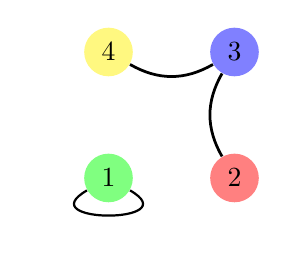
\begin{tikzpicture}
  [scale=.4,auto=left,every node/.style={circle}]
\node (n1)[fill=blue!50] at (4,4) {3};
  \node (n2)[fill=green!50] at (0,0)  {1};
  \node (n3)[fill=red!50] at (4,0)  {2};
  \node (n4)[fill=yellow!50] at (0,4)  {4};

 \path [line width=0.35mm,black] (n1) edge [bend right] (n3)
(n1) edge [bend left] (n4);
% \foreach \from/\to in {n3/n1,n1/n4}
%    \draw[black,thick] (\from) -- (\to);
     \draw[black,thick]
  (n2) to[out=210,in=330,looseness=4] (n2);
\end{tikzpicture}
\caption{The graph representing cube~3}\label{22g3}
\end{center}
\end{figure}

\begin{figure}[h]
\begin{center}
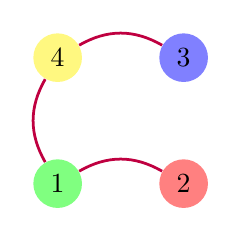
\begin{tikzpicture}
  [scale=.4,auto=left,every node/.style={circle}]
\node (n1)[fill=blue!50] at (4,4) {3};
  \node (n2)[fill=green!50] at (0,0)  {1};
  \node (n3)[fill=red!50] at (4,0)  {2};
  \node (n4)[fill=yellow!50] at (0,4)  {4};
 %\foreach \from/\to in {n3/n1,n1/n4,n2/n4}
 %   \draw[purple,thick] (\from) -- (\to);
 \path [line width=0.35mm, purple] (n2) edge [bend left] (n3)
(n1) edge [bend right] (n4)
(n2) edge [bend left] (n4);
\end{tikzpicture}
\caption{The graph representing cube~4}\label{22g4}
\end{center}
\end{figure}

Ajur was mesmerized by the graphs in front of him. He said, ``Now we need to combine these graphs, right?''

Rishnak smiled broadly. He flashed his hands and the graphs came together to form one giant graph [Figure~\ref{22g5}].

\begin{figure}[h]
\begin{center}
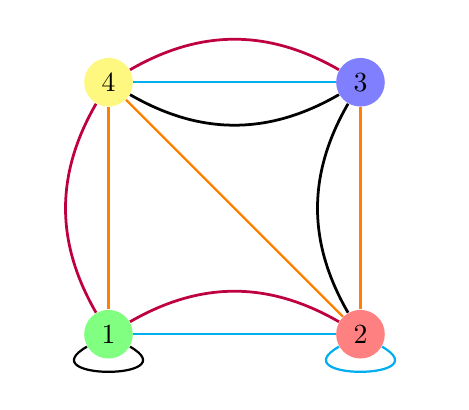
\begin{tikzpicture}
  [scale=.8,auto=left,every node/.style={circle}]
\node (n1)[fill=blue!50] at (4,4) {3};
  \node (n2)[fill=green!50] at (0,0)  {1};
  \node (n3)[fill=red!50] at (4,0)  {2};
  \node (n4)[fill=yellow!50] at (0,4)  {4};

 \foreach \from/\to in {n3/n2,n1/n4}
    \draw[cyan,thick] (\from) -- (\to);
  \draw[cyan,thick]
  (n3) to[out=210,in=330,looseness=4] (n3);
 \foreach \from/\to in {n3/n1,n3/n4,n2/n4}
    \draw[orange,thick] (\from) -- (\to); 
 \path [line width=0.35mm,black] (n1) edge [bend right] (n3)
(n1) edge [bend left] (n4);
     \draw[black,thick]
  (n2) to[out=210,in=330,looseness=4] (n2);  
   \path [line width=0.35mm, purple] (n2) edge [bend left] (n3)
(n1) edge [bend right] (n4)
(n2) edge [bend left] (n4);
\end{tikzpicture}
\caption{The graph representing all four of the cubes}\label{22g5}
\end{center}
\end{figure}

Rishnak said, ``From this graph, we need to figure out which faces of the cubes are selected as sides of the column. Essentially, there are four sides---front, back, left, and right\footnote{For this problem, the top and bottom faces are not relevant.}---and the graph in front of you has this information as a subgraph. Let us try to obtain two subgraphs with orientation so that we know the order of the sides. The first subgraph will give us the front and back faces, while the second subgraph will give us the left and right faces.''

Ajur scratched his head but continued to follow along.

Rishnak continued, ``The constraints on the subgraphs are:
\begin{enumerate}
    \item The two subgraphs should have no edge in common since an edge represents front-to-back or left-to-right, and we cannot use them for both.
    \item Each subgraph should contain an edge from each cube, which will make sure that we use all four of the cubes. In the graph, this means all of the edges should be different colors.
    \item Each vertex should have a degree of~2 in the subgraph since the colors cannot repeat.''
\end{enumerate}

Ajur tried to keep up.

Excitedly, Rishnak went on, waving his hands to form the two subgraphs [Figure~\ref{22g6}] [Figure~\ref{22g7}]. He said, ``From the original graph, we can extract these two subgraphs.''

\begin{figure}[h]
\begin{center}
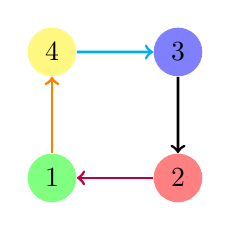
\begin{tikzpicture}
  [scale=.4,auto=left,every node/.style={circle}]
\node (n1)[fill=blue!50] at (4,4) {3};
  \node (n2)[fill=green!50] at (0,0)  {1};
  \node (n3)[fill=red!50] at (4,0)  {2};
  \node (n4)[fill=yellow!50] at (0,4)  {4};


 \path [line width=0.35mm,cyan] (n4) edge [->] (n1);
 
    \path [line width=0.35mm,orange] (n2) edge [->] (n4);
 \path [line width=0.35mm,black] (n1) edge [->] (n3);
 
   \path [line width=0.35mm, purple] (n3) edge [->] (n2);
;
\end{tikzpicture}
\caption{A subgraph depicting the front and back faces}\label{22g6}
\end{center}
\end{figure}

\begin{figure}[h]
\begin{center}
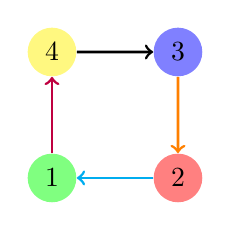
\begin{tikzpicture}
  [scale=.4,auto=left,every node/.style={circle}]
\node (n1)[fill=blue!50] at (4,4) {3};
  \node (n2)[fill=green!50] at (0,0)  {1};
  \node (n3)[fill=red!50] at (4,0)  {2};
  \node (n4)[fill=yellow!50] at (0,4)  {4};


 \path [line width=0.35mm,black] (n4) edge [->] (n1);
 
    \path [line width=0.35mm,purple] (n2) edge [->] (n4);
 \path [line width=0.35mm,orange] (n1) edge [->] (n3);
 
   \path [line width=0.35mm, cyan] (n3) edge [->] (n2);
;
\end{tikzpicture}
\caption{A subgraph depicting the left and right faces}\label{22g7}
\end{center}
\end{figure}

Rishnak continued, ``From these two subgraphs, we can figure out what colors the four sides must be. Here is the solution for each cube.
\begin{enumerate}
    \item Cube 1: front is yellow, back is blue, left is red, right is green---and this corresponds to an edge color of cyan in the subgraphs.
    \item Cube 2: front is green, back is yellow, left is blue, right is red---and this corresponds to an edge color of orange in the subgraphs.
    \item Cube 3: front is blue, back is red, left is yellow, right is blue---and this corresponds to an edge color of black in the subgraphs.
    \item Cube 4: front is red m back is green, left is green, right is yellow---and this corresponds to an edge color of purple in the subgraphs.''
\end{enumerate}

Ajur asked, ``How did you find the subgraphs with the constraints that you mentioned?''

Rishnak grinned and said, ``For a small case, we can do a visual inspection and obtain the decomposition, but in general, this is a very hard problem.''

Ajur said, ``Suppose we have four cubes, with each cube colored on all faces with the same color. So the first cube is all red, the second cube is all yellow, the third cube is all blue, and the fourth cube is all green. Then the two subgraphs will be easy to extract---and of course the solution is trivial.''

Rishnak waved his hands and four new graphs appeared [Figure~\ref{22g8}].  He said, ``Yes, here are the original four graphs. And the decomposition into two subgraphs is shown here.''

He flashed his hands again and two more figures appeared [Figure~\ref{22g9}] [Figure~\ref{22g10}].


\tikzset{every loop/.style={min distance=10mm,looseness=10}}

\begin{figure}[h]
\begin{center}
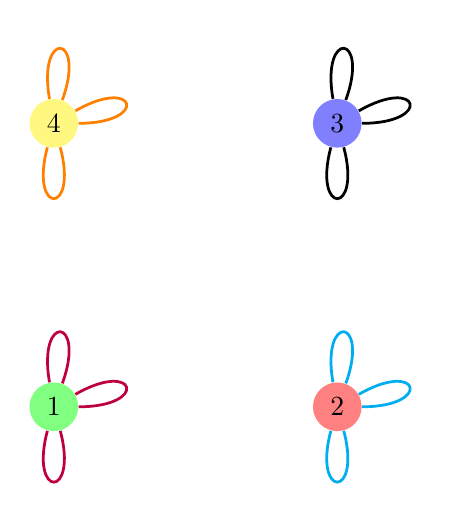
\begin{tikzpicture}
  [scale=.9,auto=left,every node/.style={circle}]
\node (n1)[fill=blue!50] at (4,4) {3};
  \node (n2)[fill=green!50] at (0,0)  {1};
  \node (n3)[fill=red!50] at (4,0)  {2};
  \node (n4)[fill=yellow!50] at (0,4)  {4};
 
 \path[line width=0.35mm, cyan] 
   (n3) edge [in=70,out=100,loop] (n3)
   (n3) edge  [in=0,out=30,loop] (n3)
   (n3) edge  [loop below] (n3); 
  \path[line width=0.35mm, orange] 
   (n4) edge [in=70,out=100,loop] (n4)
   (n4) edge  [in=0,out=30,loop] (n4)
   (n4) edge  [loop below] (n4); 
  \path[line width=0.35mm, black] 
   (n1) edge [in=70,out=100,loop] (n1)
   (n1) edge  [in=0,out=30,loop] (n1)
   (n1) edge  [loop below] (n1); 
  \path[line width=0.35mm, purple] 
   (n2) edge [in=70,out=100,loop] (n2)
   (n2) edge  [in=0,out=30,loop] (n2)
   (n2) edge  [loop below] (n2); 
   
\end{tikzpicture}
\caption{A graph for all four of the cubes}\label{22g8}
\end{center}
\end{figure}

\begin{figure}[h]
\begin{center}
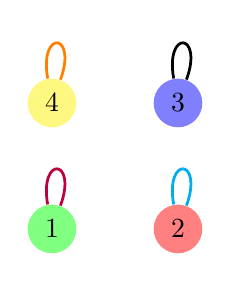
\begin{tikzpicture}
  [scale=.4,auto=left,every node/.style={circle}]
\node (n1)[fill=blue!50] at (4,4) {3};
  \node (n2)[fill=green!50] at (0,0)  {1};
  \node (n3)[fill=red!50] at (4,0)  {2};
  \node (n4)[fill=yellow!50] at (0,4)  {4};
 
 \path[line width=0.35mm, cyan] 
   (n3) edge [in=70,out=100,loop] (n3);
   
  \path[line width=0.35mm, orange] 
   (n4) edge [in=70,out=100,loop] (n4);
  
  \path[line width=0.35mm, black] 
   (n1) edge [in=70,out=100,loop] (n1);
  
  \path[line width=0.35mm, purple] 
   (n2) edge [in=70,out=100,loop] (n2);
    
   
\end{tikzpicture}
\caption{A subgraph for the graph shown in Figure~\ref{22g8} representing the front and back faces}\label{22g9}
\end{center}
\end{figure}
\begin{figure}[h]
\begin{center}
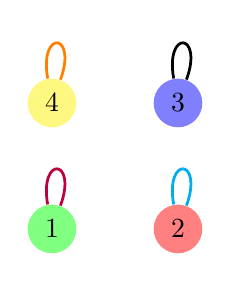
\begin{tikzpicture}
  [scale=.4,auto=left,every node/.style={circle}]
\node (n1)[fill=blue!50] at (4,4) {3};
  \node (n2)[fill=green!50] at (0,0)  {1};
  \node (n3)[fill=red!50] at (4,0)  {2};
  \node (n4)[fill=yellow!50] at (0,4)  {4};
 
 \path[line width=0.35mm, cyan] 
   (n3) edge [in=70,out=100,loop] (n3);
   
  \path[line width=0.35mm, orange] 
   (n4) edge [in=70,out=100,loop] (n4);
  
  \path[line width=0.35mm, black] 
   (n1) edge [in=70,out=100,loop] (n1);
  
  \path[line width=0.35mm, purple] 
   (n2) edge [in=70,out=100,loop] (n2);
    
   
\end{tikzpicture}
\caption{A subgraph for the graph shown in Figure~\ref{22g8} representing the left and right faces}\label{22g10}
\end{center}
\end{figure}

Before Rishnak could speak further, Ajur quickly said, ``Aha, the solution is then this.
\begin{enumerate}
    \item Cube 1: front is red, back is red, left is red, right is red.
    \item Cube 2: front is yellow, back is yellow, left is yellow, right is yellow.
    \item Cube 3: front is blue, back is blue, left is blue, right is blue.
    \item Cube 4: front is green, back is green, left is green, right is green.''
\end{enumerate}

By this time, from the past nineteen days, Ajur felt he had a very clear understanding of all of the concepts of graph theory they had covered, as well as a desire to keep learning more.

He faced Rishnak and said, ``Rishnak, thank you for teaching me and helping me understand all of these wonderfully interesting problems.''

Rishnak blushed (if that is possible for a ghost).

\subsection*{Question for the twentieth day}
After a few moments, Rishnak said, ``At long last, we have arrived at the twentieth day. I have one last question for you, Ajur. I hope you can answer it, as it will also set me free.''

Ajur took a deep breath and said, ``I will do my best.''

Rishnak said, ``Can you decompose this graph''---Rishnak flashed his hands and a final graph appeared [Figure~\ref{22q1}]---``for all new sets of cubes by drawing the color of one face of one of the cubes?''

\begin{figure}[h]
\begin{center}
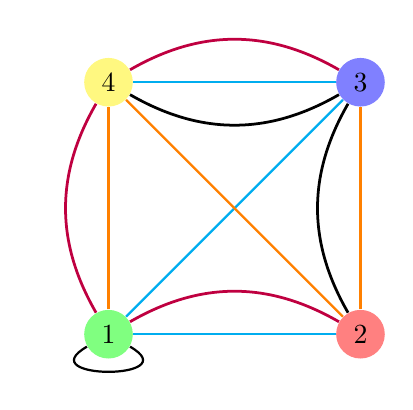
\begin{tikzpicture}
  [scale=.8,auto=left,every node/.style={circle}]
\node (n1)[fill=blue!50] at (4,4) {3};
  \node (n2)[fill=green!50] at (0,0)  {1};
  \node (n3)[fill=red!50] at (4,0)  {2};
  \node (n4)[fill=yellow!50] at (0,4)  {4};

 \foreach \from/\to in {n2/n1,n1/n4,n2/n3}
    \draw[cyan,thick] (\from) -- (\to);
 
 \foreach \from/\to in {n3/n1,n3/n4,n2/n4}
    \draw[orange,thick] (\from) -- (\to); 
 \path [line width=0.35mm,black] (n1) edge [bend right] (n3)
(n1) edge [bend left] (n4);
     \draw[black,thick]
  (n2) to[out=210,in=330,looseness=4] (n2);  
   \path [line width=0.35mm, purple] (n2) edge [bend left] (n3)
(n1) edge [bend right] (n4)
(n2) edge [bend left] (n4);
\end{tikzpicture}
\caption{A graph for all of the new cubes}\label{22q1}
\end{center}
\end{figure}

\textit{Before you turn the page, try to come up with answers of your own!}

\newpage
\subsection*{Answer for the twentieth day}
Ajur tried to decompose the graphs using the same approach as before.
Before long, he drew two final subgraphs in the dirt [Figure~\ref{22ga2}] [Figure~\ref{22ga3}].
He said, ``Here are the two subgraphs, Rishnak.''

\begin{figure}[h]
\begin{center}
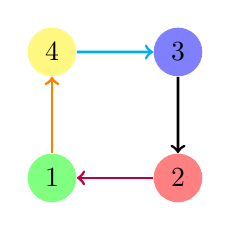
\begin{tikzpicture}
  [scale=.4,auto=left,every node/.style={circle}]
\node (n1)[fill=blue!50] at (4,4) {3};
  \node (n2)[fill=green!50] at (0,0)  {1};
  \node (n3)[fill=red!50] at (4,0)  {2};
  \node (n4)[fill=yellow!50] at (0,4)  {4};


 \path [line width=0.35mm,cyan] (n4) edge [->] (n1);
 
    \path [line width=0.35mm,orange] (n2) edge [->] (n4);
 \path [line width=0.35mm,black] (n1) edge [->] (n3);
 
   \path [line width=0.35mm, purple] (n3) edge [->] (n2);
;
\end{tikzpicture}
\caption{The subgraph from the graph in Figure~\ref{22q1} depicting the front and back faces}\label{22ga2}
\end{center}
\end{figure}

\begin{figure}[h]
\begin{center}
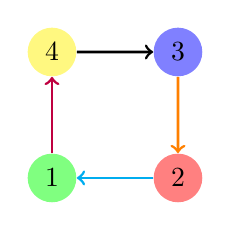
\begin{tikzpicture}
  [scale=.4,auto=left,every node/.style={circle}]
\node (n1)[fill=blue!50] at (4,4) {3};
  \node (n2)[fill=green!50] at (0,0)  {1};
  \node (n3)[fill=red!50] at (4,0)  {2};
  \node (n4)[fill=yellow!50] at (0,4)  {4};


 \path [line width=0.35mm,black] (n4) edge [->] (n1);
 
    \path [line width=0.35mm,purple] (n2) edge [->] (n4);
 \path [line width=0.35mm,orange] (n1) edge [->] (n3);
 
   \path [line width=0.35mm, cyan] (n3) edge [->] (n2);
;
\end{tikzpicture}
\caption{The subgraph from the graph in Figure~\ref{22q1} depicting the left and right faces}\label{22ga3}
\end{center}
\end{figure}

Rishnak smiled like he had never smiled before. He said, ``Correct.''

Ajur smiled back and said, ``Thank you, Rishnak.''

Ajur and Jura said their goodbyes to Rishnak. Not far away, Kinaja watched, smiling to herself that Ajur not only understood the concepts but also had the decency to thank Rishnak for all of his efforts.
